\documentclass[]{article}
\usepackage{lmodern}
\usepackage{amssymb,amsmath}
\usepackage{ifxetex,ifluatex}
\usepackage{fixltx2e} % provides \textsubscript
\ifnum 0\ifxetex 1\fi\ifluatex 1\fi=0 % if pdftex
  \usepackage[T1]{fontenc}
  \usepackage[utf8]{inputenc}
\else % if luatex or xelatex
  \ifxetex
    \usepackage{mathspec}
    \usepackage{xltxtra,xunicode}
  \else
    \usepackage{fontspec}
  \fi
  \defaultfontfeatures{Mapping=tex-text,Scale=MatchLowercase}
  \newcommand{\euro}{€}
\fi
% use upquote if available, for straight quotes in verbatim environments
\IfFileExists{upquote.sty}{\usepackage{upquote}}{}
% use microtype if available
\IfFileExists{microtype.sty}{%
\usepackage{microtype}
\UseMicrotypeSet[protrusion]{basicmath} % disable protrusion for tt fonts
}{}
\usepackage[margin=1in]{geometry}
\usepackage{color}
\usepackage{fancyvrb}
\newcommand{\VerbBar}{|}
\newcommand{\VERB}{\Verb[commandchars=\\\{\}]}
\DefineVerbatimEnvironment{Highlighting}{Verbatim}{commandchars=\\\{\}}
% Add ',fontsize=\small' for more characters per line
\usepackage{framed}
\definecolor{shadecolor}{RGB}{248,248,248}
\newenvironment{Shaded}{\begin{snugshade}}{\end{snugshade}}
\newcommand{\KeywordTok}[1]{\textcolor[rgb]{0.13,0.29,0.53}{\textbf{{#1}}}}
\newcommand{\DataTypeTok}[1]{\textcolor[rgb]{0.13,0.29,0.53}{{#1}}}
\newcommand{\DecValTok}[1]{\textcolor[rgb]{0.00,0.00,0.81}{{#1}}}
\newcommand{\BaseNTok}[1]{\textcolor[rgb]{0.00,0.00,0.81}{{#1}}}
\newcommand{\FloatTok}[1]{\textcolor[rgb]{0.00,0.00,0.81}{{#1}}}
\newcommand{\CharTok}[1]{\textcolor[rgb]{0.31,0.60,0.02}{{#1}}}
\newcommand{\StringTok}[1]{\textcolor[rgb]{0.31,0.60,0.02}{{#1}}}
\newcommand{\CommentTok}[1]{\textcolor[rgb]{0.56,0.35,0.01}{\textit{{#1}}}}
\newcommand{\OtherTok}[1]{\textcolor[rgb]{0.56,0.35,0.01}{{#1}}}
\newcommand{\AlertTok}[1]{\textcolor[rgb]{0.94,0.16,0.16}{{#1}}}
\newcommand{\FunctionTok}[1]{\textcolor[rgb]{0.00,0.00,0.00}{{#1}}}
\newcommand{\RegionMarkerTok}[1]{{#1}}
\newcommand{\ErrorTok}[1]{\textbf{{#1}}}
\newcommand{\NormalTok}[1]{{#1}}
\usepackage{longtable,booktabs}
\usepackage{graphicx}
\makeatletter
\def\maxwidth{\ifdim\Gin@nat@width>\linewidth\linewidth\else\Gin@nat@width\fi}
\def\maxheight{\ifdim\Gin@nat@height>\textheight\textheight\else\Gin@nat@height\fi}
\makeatother
% Scale images if necessary, so that they will not overflow the page
% margins by default, and it is still possible to overwrite the defaults
% using explicit options in \includegraphics[width, height, ...]{}
\setkeys{Gin}{width=\maxwidth,height=\maxheight,keepaspectratio}
\ifxetex
  \usepackage[setpagesize=false, % page size defined by xetex
              unicode=false, % unicode breaks when used with xetex
              xetex]{hyperref}
\else
  \usepackage[unicode=true]{hyperref}
\fi
\hypersetup{breaklinks=true,
            bookmarks=true,
            pdfauthor={Lisa MALIPHOL},
            pdftitle={~Exploratory Data Analysis Virtual SCADA Network:},
            colorlinks=true,
            citecolor=blue,
            urlcolor=blue,
            linkcolor=magenta,
            pdfborder={0 0 0}}
\urlstyle{same}  % don't use monospace font for urls
\setlength{\parindent}{0pt}
\setlength{\parskip}{6pt plus 2pt minus 1pt}
\setlength{\emergencystretch}{3em}  % prevent overfull lines
\setcounter{secnumdepth}{0}

%%% Use protect on footnotes to avoid problems with footnotes in titles
\let\rmarkdownfootnote\footnote%
\def\footnote{\protect\rmarkdownfootnote}

%%% Change title format to be more compact
\usepackage{titling}
\setlength{\droptitle}{-2em}
  \title{~Exploratory Data Analysis\\Virtual SCADA Network:}
  \pretitle{\vspace{\droptitle}\centering\huge}
  \posttitle{\par}
  \author{Lisa MALIPHOL}
  \preauthor{\centering\large\emph}
  \postauthor{\par}
  \date{}
  \predate{}\postdate{}




\begin{document}

\maketitle


\section{Introduction}\label{introduction}

As a first step in the SCAD@COPS project presented in its introduction
{[}1{]}, the initial phase of exploratory data analysis is conducted in
order to be able to better understand the data. In addition to the
traditional methods of using descriptive statistics to explain the data,
the various graphical and visual manners of representing the data are
presented.

The paper is an analysis and statistical study of network traffic
captured over a virtual SCADA network with simulated attacks. The
network traffic was captured using Wireshark, and R was the language
used to carry out the statistical analysis. The organisation of this
study is presented in the following sections-

The paper is organized as follows:

\begin{itemize}
\itemsep1pt\parskip0pt\parsep0pt
\item
  Tools used during this process
\item
  Data source
\item
  Exploratory Data Analysis

  \begin{itemize}
  \itemsep1pt\parskip0pt\parsep0pt
  \item
    Statistical definitions
  \item
    Visual representations defined
  \item
    Analysis
  \end{itemize}
\end{itemize}

\section{Tools}\label{tools}

A great deal of work is typically involved in preparing the raw data for
analysis. Depending on the initial state of the data, various
pre-processing and transformations may be required. The following tools
were used in the exploratory phase of data analysis in order to capture,
transform and analyze the data. The commands and scripts used in this
process are found in Appendix B.

\subsection[Wireshark - Network Traffic Analysis
Tool]{Wireshark\footnote{\url{https://www.wireshark.org/docs/wsug_html_chunked}}
- Network Traffic Analysis
Tool}\label{wireshark1---network-traffic-analysis-tool}

Developed in 1997 by Gerald Combs originally named Ethereal, Wireshark
is now an Open Source GNU project. It is a network packet analyzer, or
``packet sniffer'', that captures and displays network packets.

Captured network packets are saved in the pcap file format and can be
dissected and parsed by Wireshark in order to analyze its contents. An
important aspect of Wireshark is that of its passive/monitoring nature
and so does not send, manipulate, or modify the data passing over the
network.

An initial packet capture file was created over simulated network
traffic using Wireshark. Using its export facilities, various files were
created for further analysis, with information such as TCP endpoints,
conversations, etc.

\subsection[TShark]{TShark\footnote{\url{https://www.wireshark.org/docs/man-pages/tshark.html}}}\label{tshark2}

Another tool from the Wireshark suite is the command-line tool similar
to tcpdump is tshark, a network protocol analyzer. In addition to
capturing packet data over a live network, it is also capable of
analyzing packets from an existing capture file. TShark was used to
parse out various pertinent variables pertaining to the Modbus/TCP
application protocol enclosed in the packet data.

\subsection{UNIX Utilities}\label{unix-utilities}

In order to further parse and transform the data, the UNIX utility tool
sed, which supports the use of regular expressions, was also used.

\subsection[R - Statistical Tool]{R - Statistical Tool\footnote{\url{http://www.r-project.org/}}}\label{r---statistical-tool3}

R is an Open Source programming language and environment used for
statistical computing and graphics. Initially developed by John Chambers
at Bell Labs as the S language in 1993, R was created as a freely
available version under the GNU project by Ross Ihaka and Robert
Gentleman at the University of Auckland, New Zealand.

Maintained by the R Development Core Team and with an active and growing
community, it provides various statistical and graphical creation
capabilities available under most operating systems, and is extensible
with numerous packages available.

\section{Data Source}\label{data-source}

\subsection[PCap File]{PCap\footnote{\url{http://www.winpcap.org/ntar/draft/PCAP-DumpFileFormat.html}}
File}\label{pcap4-file}

A packet capture file was created via Wireshark, which captured the
network traffic simulated over a virtual SCADA network. This file also
included injected random attacks over the network.

\begin{longtable}[c]{@{}ll@{}}
\toprule
SCADA\_Security\_042915.pcap &\tabularnewline
\midrule
\endhead
File &\tabularnewline
Length: & 271279028 bytes\tabularnewline
Format: & Wireshark/tcpdump/\ldots{} - libcap\tabularnewline
Encapsulation: & Ethernet\tabularnewline
Packet size limit: & 65536\tabularnewline
Time &\tabularnewline
First packet: & 2015-04-29 12:51:40\tabularnewline
Last packet: & 2015-04-29 17:28:37\tabularnewline
Elapsed: & 04:36:56\tabularnewline
Traffic Captured &\tabularnewline
Packets & 3566852\tabularnewline
B/t first and last pkt & 16616,418 sec\tabularnewline
Avg. packets/sec & 214,661\tabularnewline
Avg. packet size & 60,055 bytes\tabularnewline
Bytes & 214208732\tabularnewline
Avg. bytes/sec & 12891,390\tabularnewline
Avg. Mit/sec & 0,103\tabularnewline
\bottomrule
\end{longtable}

Once the network traffic was captured and saved in a pcap file,
Wireshark provides the capability to export the raw data into various
comma delimited files in order to do further analysis. Exported files
were created with TCP endpoints, TCP conversations, as well as the
entire pcap file, each as a CSV file. (Appendix A)

\section{Exploratory Data Analysis}\label{exploratory-data-analysis}

Originally championed by John Tukey{[}2{]}, Exploratory Data Analysis
(EDA) is an initial approach to understanding a data set in order to get
a ``feel'' for the data, to summarizing its essential characteristics
and to studying patterns in the data. In addition to using quantitative
techniques, it is supported predominantly by means of graphical
representations.

Conducting EDA possibly gives further insight into the form and
structure of the data set, in addition to extracting value from it,
visualizing it, and just as importantly, in communicating it.

Following are some brief explanations of descriptive statistical terms,
as well as the graphical representations used.

\subsection{Statistical Definitions}\label{statistical-definitions}

\subsubsection{Mean}\label{mean}

The (arithmetic) mean is a measure of central tendency, which is a
single value which represents an average of the sample or population. It
is calculated by dividing all the observations by the number of
observations.

\subsubsection{Median}\label{median}

Another measure of central tendency is the median, however, in this
case, the median is determined by first ordering the observations by
magnitude. Then the median is taken as the value which falls in the
middle, or the average of the two middle values in the case of an even
number of observations. The median is better suited when there are
observations, or outliers, that fall way outside the norm. These are
extreme values that differ greatly from other values in the data set.

\subsubsection{Variance}\label{variance}

The variance is the expected value of the squared differences between
the random variables and its mean that is always positive. It gives an
indication of how far apart the values are from the mean and each other.
\[ var[X] = E[(X - E[X])^2] \]

\subsubsection{Standard Deviation}\label{standard-deviation}

The standard deviation is a measure of dispersion, or how spread out a
random variable is around its mean. It is calculated as the square root
of the variance and is, unlike the variance, expressed in the same terms
as the data. \[ std[X] = \sqrt(var[X]) \]

\subsubsection{Covariance}\label{covariance}

A measure of how closely two variables change, or vary together is the
covariance. Random random variables whose covariance is 0 is said to be
uncorrelated. \[ cov[X,Y] = E[(X - E[X])(Y-E[Y])] \]

\subsubsection{Correlation}\label{correlation}

Correlation is the strength between the relationship of, or dependence
between, two variables whose value is typically bounded between the
values of -1 and 1, that is to say, that the value has been normalized.
It describes the magnitude and the direction of the relationship. If the
correlation is positive, their values increase together, and if it is
negative, one value decreases as the other value increases.
\[ corr[X,Y] = cov[X,Y] / (std[X]std[Y]) \]

\subsection{Visual Representations}\label{visual-representations}

\subsubsection{Pie chart}\label{pie-chart}

A pie chart is a circular diagram representing numerical proportions as
slices of the pie. Scatter plot A diagram showing a collection of points
as depicted by the coordinates between (typically) two variables on a
plane. One axis represents the independent variable, whereas the other
represents the dependent variable.

\subsubsection{Histogram}\label{histogram}

A graphical representation which shows the distribution of continuous
numerical values is a histogram and can be representative of a
probability distribution. A frequency histogram is a univariate
graphical way to show frequency counts of a value depicted with bars of
different heights.

\subsubsection{Bar chart}\label{bar-chart}

Similar to a histogram, a bar chart shows the distribution of values of
a given variable,however, the data is in categorized.

\subsubsection{Boxplot}\label{boxplot}

An effective and graphical method for visualizing outliers is the
boxplot. It displays the data in terms of interquartiles, where outliers
are depicted as individual points. (Boxplot image source{[}3{]})

\begin{center}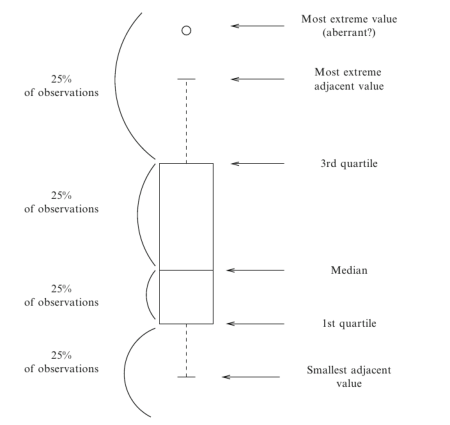
\includegraphics{edaReport_files/figure-latex/unnamed-chunk-2-1} \end{center}

\subsubsection{Heat Map}\label{heat-map}

A heat map displays data in a matrix where the values are represented by
a range of colors. Typically displayed in 2D, larger values are usually
shown in darker colors and smaller values in lighter colors on a heat
map. They can also be accompanied by a dendrogram, a tree diagram used
to illustrate clusters.

\subsubsection{Network Graph}\label{network-graph}

Used to model relations between objects, another mathematical structure
is the graph, comprised of nodes, or vertices, and edges. Depending on
the nature of the relationship, a graph may be either cyclic or acyclic,
directed or undirected. Attributes of a node or edge may be reflected in
the graph as well.

\subsection{Analysis}\label{analysis}

\subsubsection{Protocols}\label{protocols}

\begin{verbatim}
##         Protocol   Count
##  1:          TCP 1692588
##  2:   Modbus/TCP  825521
##  3:          ARP  751226
##  4:        T.125  277283
##  5:         HTTP   11275
##  6:          DNS    2525
##  7:          SMB    1007
##  8:          UDP     861
##  9:         IMAP     849
## 10:        TLSv1     575
## 11:         SMTP     533
## 12:         ICMP     526
## 13:         NBNS     491
## 14:       PN-DCP     364
## 15:       DHCPv6     273
## 16:       Syslog     246
## 17:      BROWSER     181
## 18:         SSDP     168
## 19:        LLMNR     128
## 20:       LANMAN     108
## 21:         NBSS      80
## 22:         MDNS      28
## 23:       DCERPC      21
## 24: RELOAD Frame      14
## 25:       REMACT       6
## 26:       SRVSVC       6
## 27:          IMF       5
## 28:         TPKT       4
##         Protocol   Count
\end{verbatim}

\begin{center}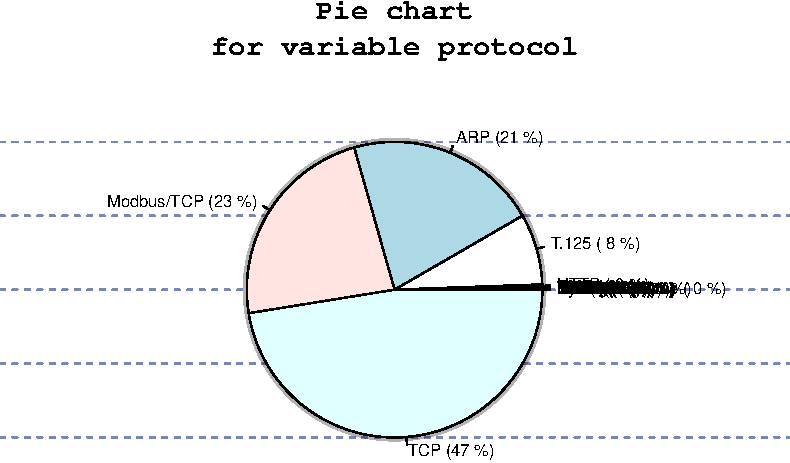
\includegraphics{edaReport_files/figure-latex/unnamed-chunk-4-1} \end{center}

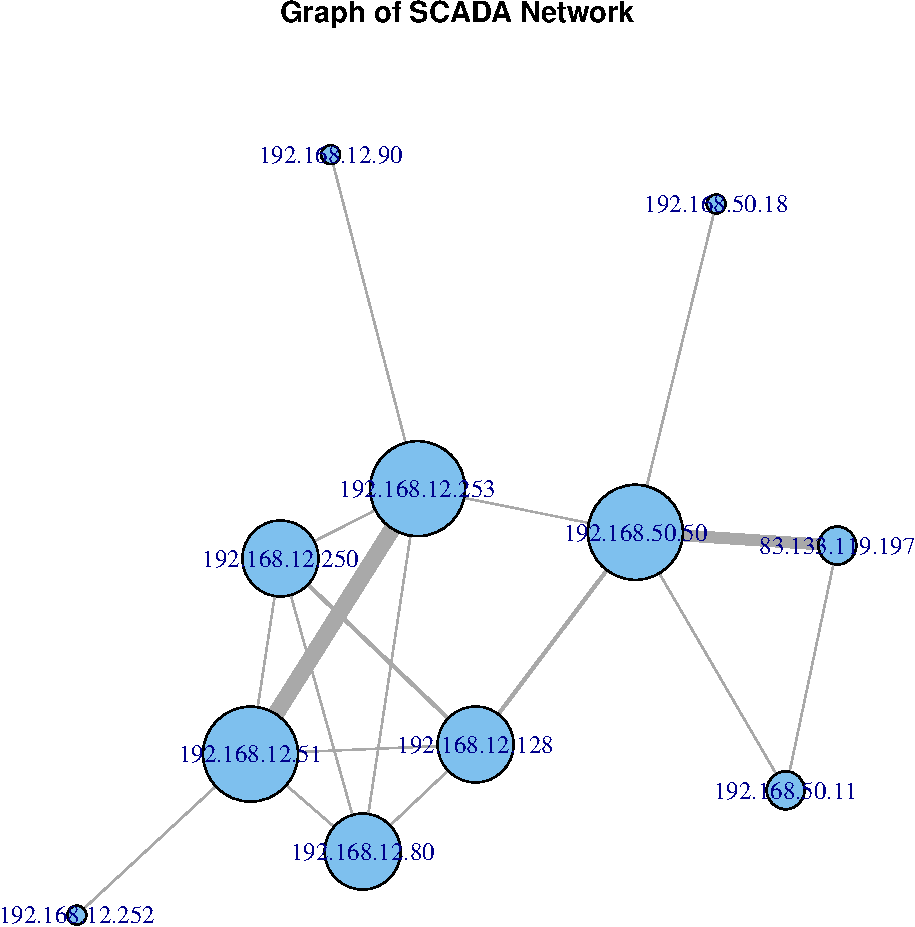
\includegraphics{edaReport_files/figure-latex/unnamed-chunk-5-1.pdf}

In the network graph shown above, the size of the node is according to
its degree of centrality, that is, the number of adjacent vertices. The
thicker edges indicate a higher number of interactions between two
nodes.

\begin{longtable}[c]{@{}ll@{}}
\toprule
Node IP Addresses &\tabularnewline
\midrule
\endhead
192.168.12.253 & Schneider\tabularnewline
192.168.12.51 & HMI\tabularnewline
192.168.50.50 &\tabularnewline
83.133.119.197 &\tabularnewline
192.168.12.80 &\tabularnewline
192.168.12.250 &\tabularnewline
192.168.12.128 &\tabularnewline
192.168.50.11 &\tabularnewline
192.168.50.18 &\tabularnewline
192.168.12.90 &\tabularnewline
192.168.12.252 &\tabularnewline
\bottomrule
\end{longtable}

\subsubsection{Packet Length Statistics}\label{packet-length-statistics}

\begin{Shaded}
\begin{Highlighting}[]
\KeywordTok{summary}\NormalTok{(scadaDT[.(}\DataTypeTok{Protocol=}\StringTok{"TCP"}\NormalTok{),.(Length)])}
\end{Highlighting}
\end{Shaded}

\begin{verbatim}
##      Length       
##  Min.   :  54.00  
##  1st Qu.:  54.00  
##  Median :  54.00  
##  Mean   :  58.09  
##  3rd Qu.:  54.00  
##  Max.   :1514.00
\end{verbatim}

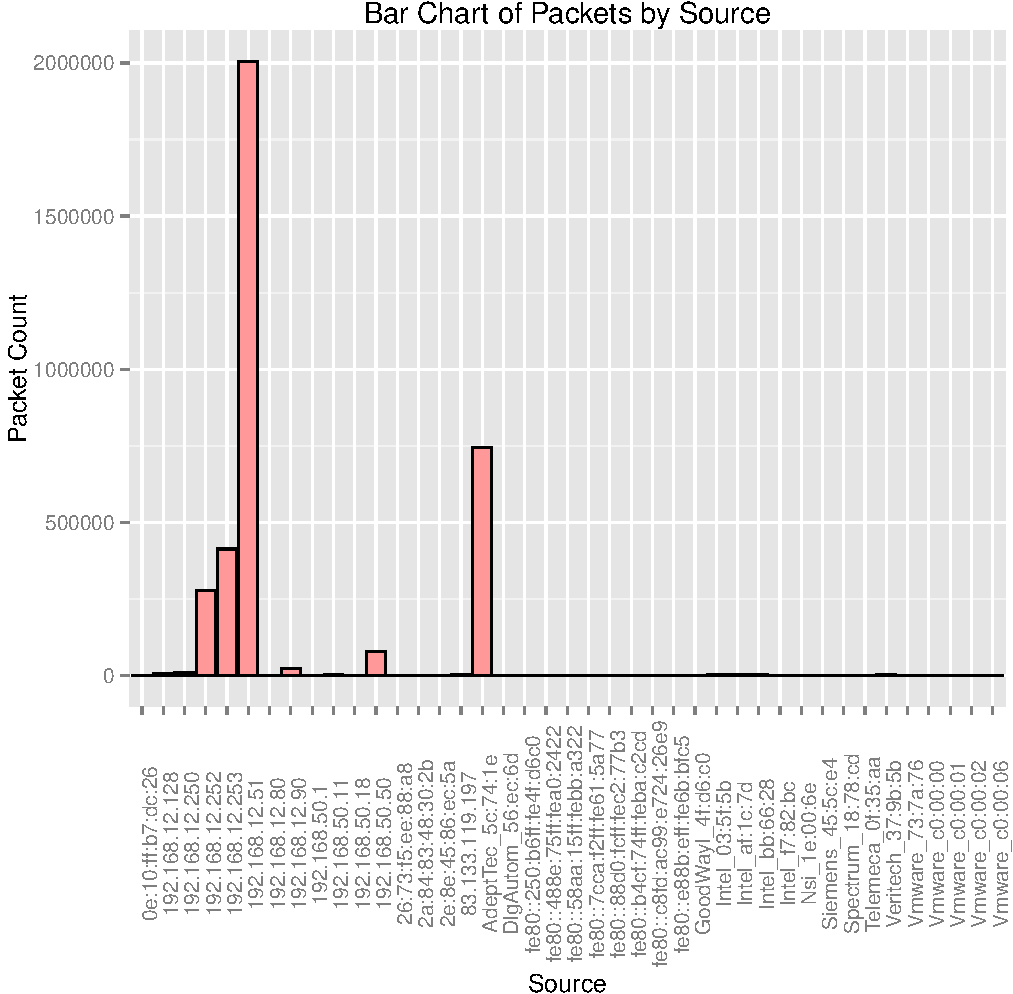
\includegraphics{edaReport_files/figure-latex/unnamed-chunk-8-1.pdf}

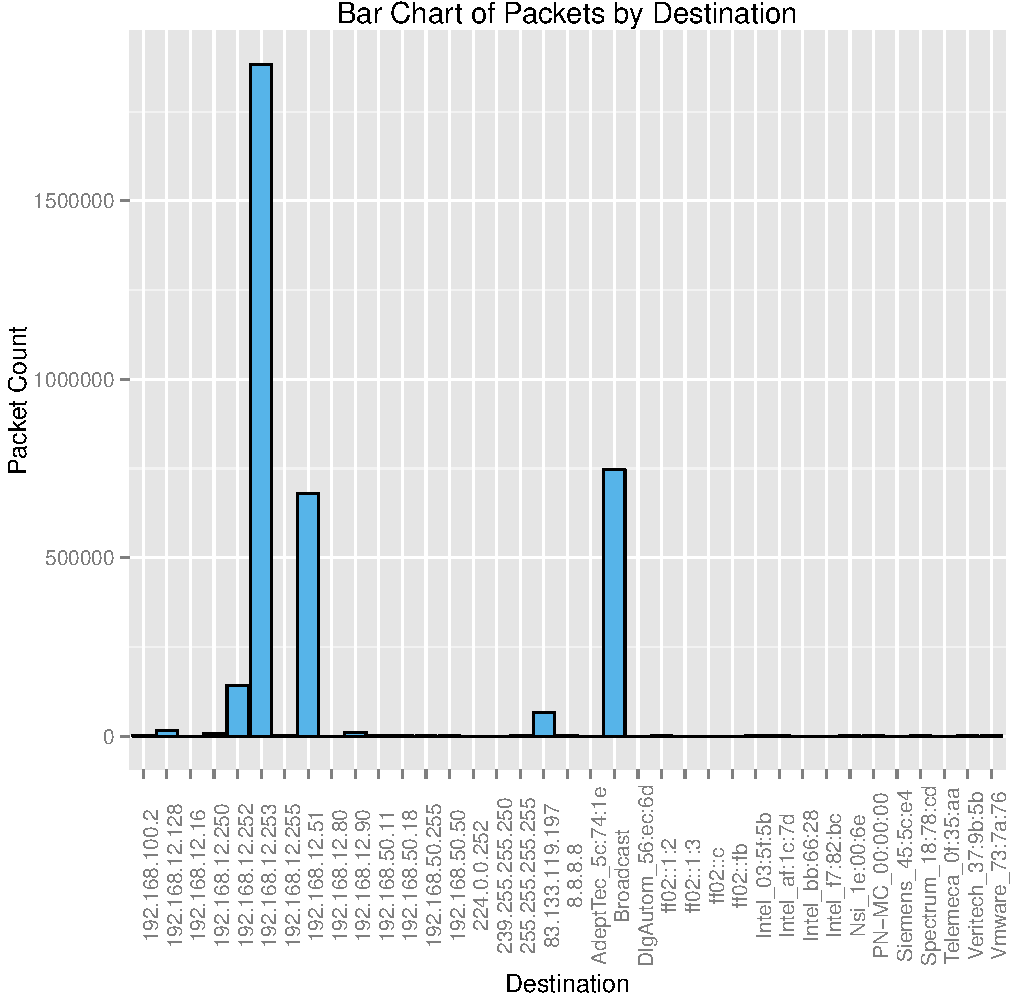
\includegraphics{edaReport_files/figure-latex/unnamed-chunk-9-1.pdf}

\pagebreak

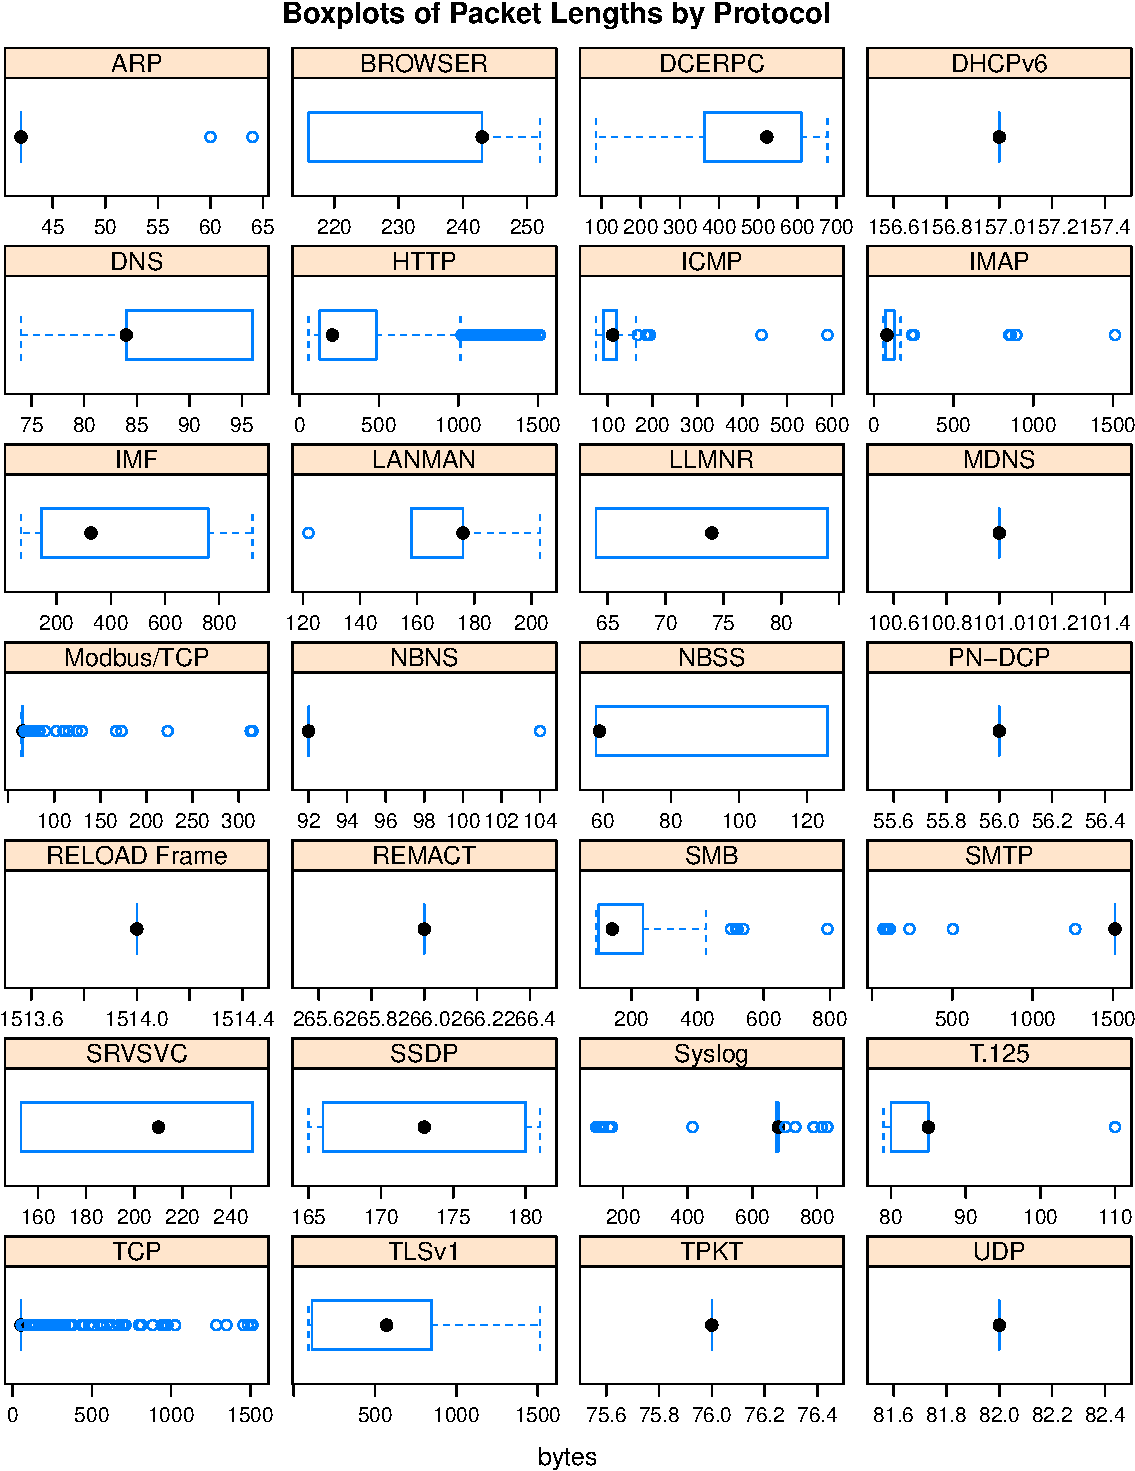
\includegraphics{edaReport_files/figure-latex/unnamed-chunk-10-1.pdf}

\pagebreak

\subsubsection{Modbus/TCP Statistics}\label{modbustcp-statistics}

\begin{Shaded}
\begin{Highlighting}[]
\KeywordTok{summary}\NormalTok{(scadaDT[.(}\DataTypeTok{Protocol=}\StringTok{"Modbus/TCP"}\NormalTok{),.(Length)])}
\end{Highlighting}
\end{Shaded}

\begin{verbatim}
##      Length     
##  Min.   : 64.0  
##  1st Qu.: 65.0  
##  Median : 66.0  
##  Mean   : 65.7  
##  3rd Qu.: 66.0  
##  Max.   :315.0
\end{verbatim}

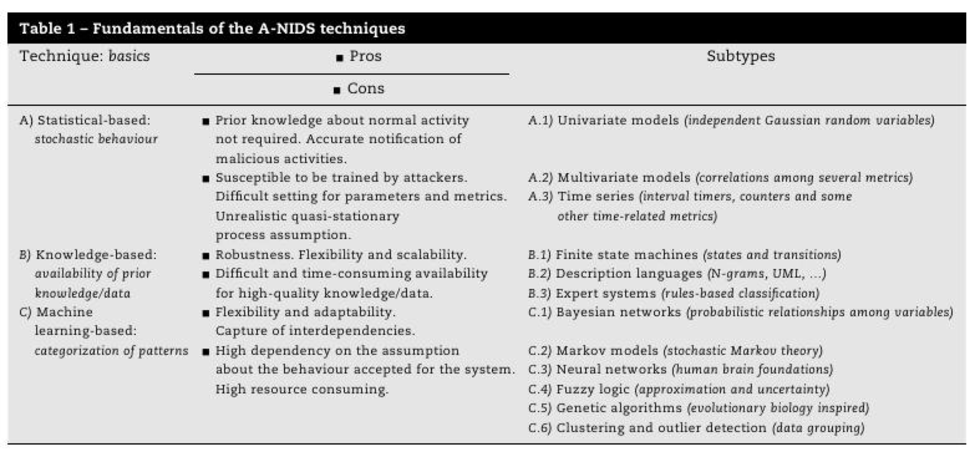
\includegraphics{edaReport_files/figure-latex/unnamed-chunk-12-1.pdf}

\begin{center}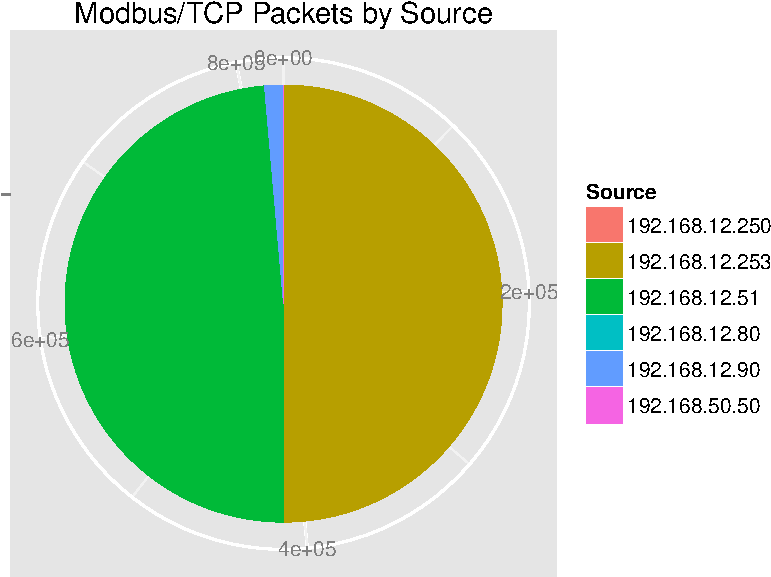
\includegraphics{edaReport_files/figure-latex/unnamed-chunk-13-1} \end{center}

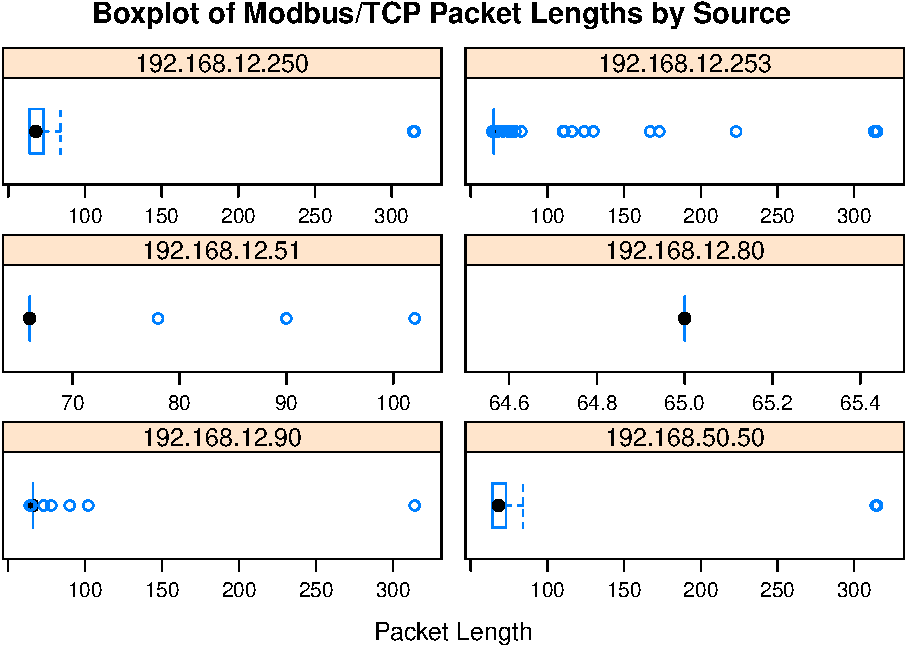
\includegraphics{edaReport_files/figure-latex/unnamed-chunk-14-1.pdf}

\begin{center}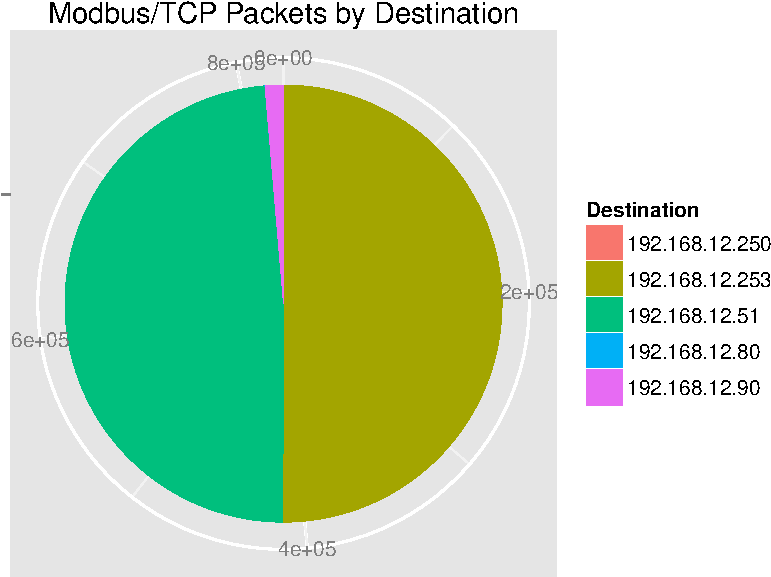
\includegraphics{edaReport_files/figure-latex/unnamed-chunk-15-1} \end{center}

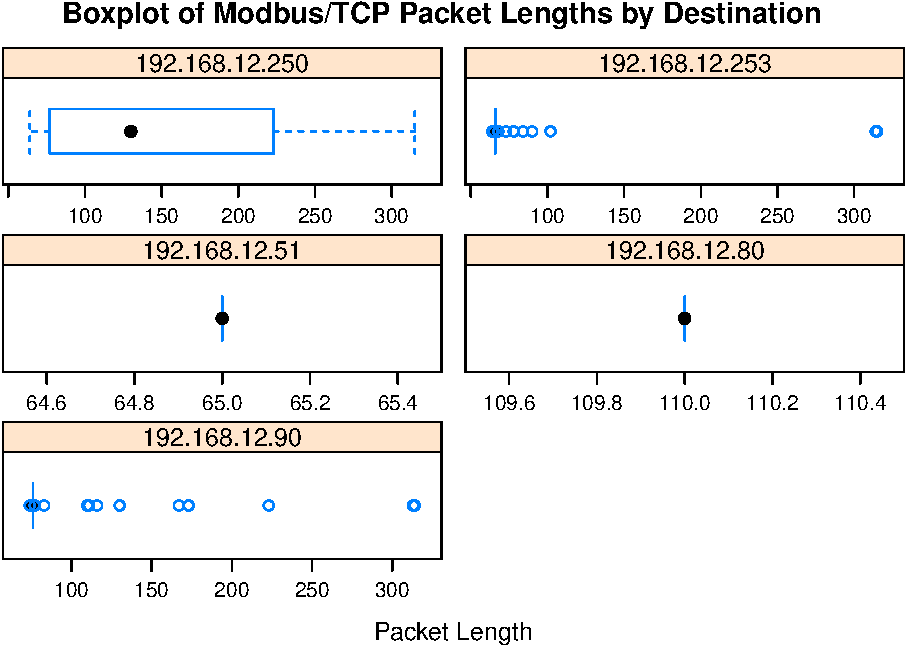
\includegraphics{edaReport_files/figure-latex/unnamed-chunk-16-1.pdf}

\subsubsection{Endpoints}\label{endpoints}

SCADA\_Security\_042915\_TCP\_Endpoints.csv

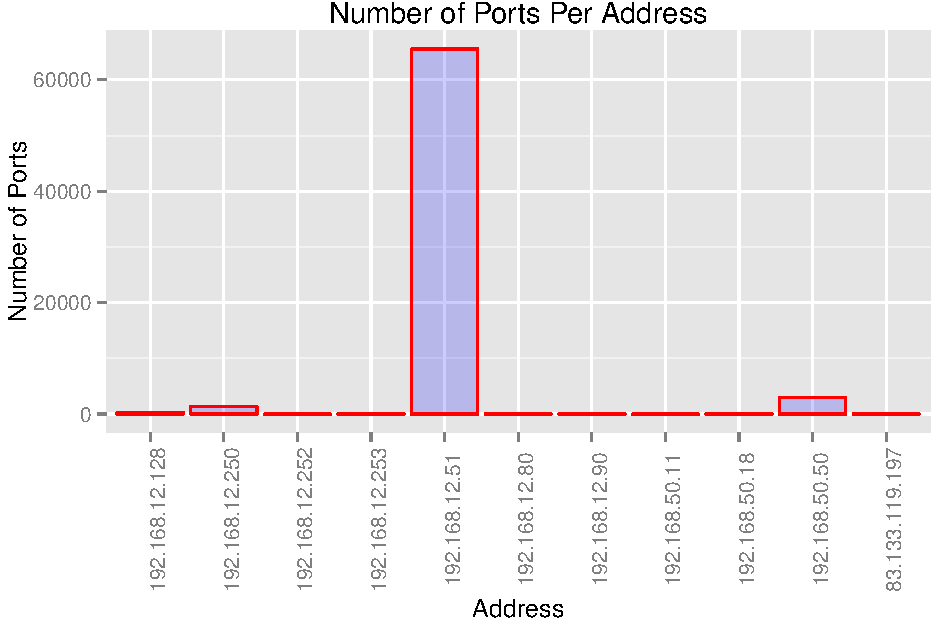
\includegraphics{edaReport_files/figure-latex/unnamed-chunk-17-1.pdf}

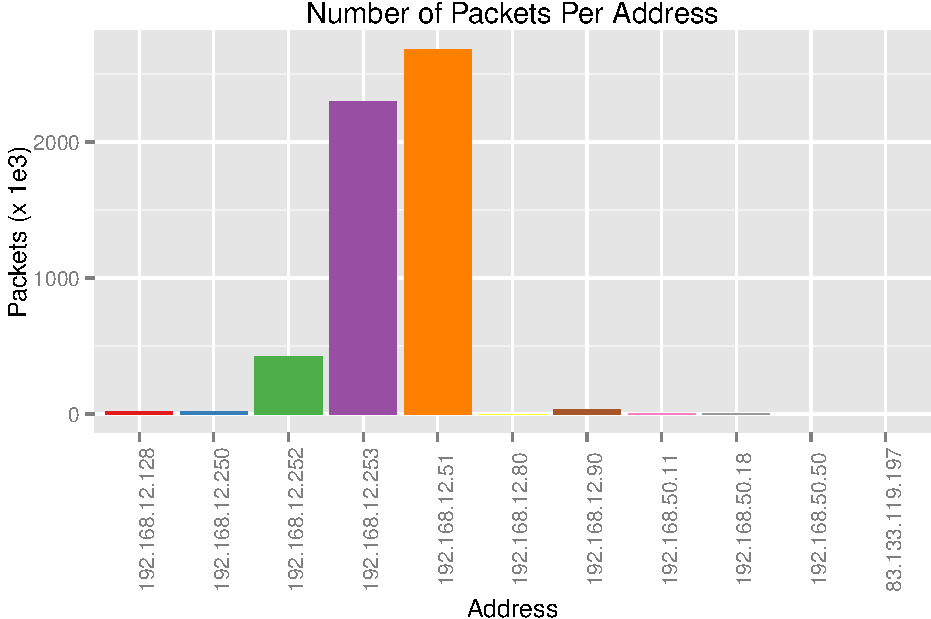
\includegraphics{edaReport_files/figure-latex/unnamed-chunk-18-1.pdf}

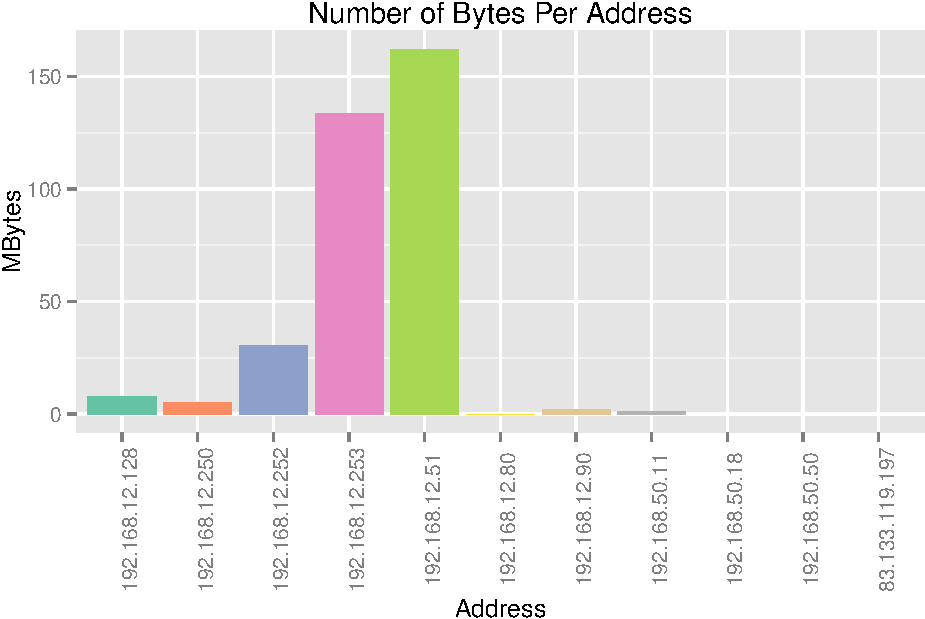
\includegraphics{edaReport_files/figure-latex/unnamed-chunk-19-1.pdf}

\subsubsection{Correlation and
Covariance}\label{correlation-and-covariance}

\begin{Shaded}
\begin{Highlighting}[]
\KeywordTok{cor}\NormalTok{(packets, }\DataTypeTok{use=}\StringTok{"complete.obs"}\NormalTok{,}\DataTypeTok{method=}\StringTok{"spearman"}\NormalTok{)}
\end{Highlighting}
\end{Shaded}

\begin{verbatim}
##                   Packets       Bytes Packets.A.B  Bytes.A.B Packets.A.B.1
## Packets        1.00000000  0.97894124   0.9788233  0.5040848    0.89660460
## Bytes          0.97894124  1.00000000   0.9165046  0.4720734    0.92313903
## Packets.A.B    0.97882329  0.91650460   1.0000000  0.5149616    0.83109826
## Bytes.A.B      0.50408481  0.47207338   0.5149616  1.0000000    0.42692965
## Packets.A.B.1  0.89660460  0.92313903   0.8310983  0.4269296    1.00000000
## Bytes.A.B.1    0.40776399  0.42066174   0.3770389 -0.5593192    0.47568586
## Duration      -0.04869179 -0.02865136  -0.0669847 -0.2816442    0.02599502
## bps.A.B        0.27557708  0.25036473   0.2899822  0.7759541    0.19682668
## bps.A.B.1      0.25341226  0.22904557   0.2673998 -0.3608199    0.19145965
##               Bytes.A.B.1    Duration    bps.A.B  bps.A.B.1
## Packets         0.4077640 -0.04869179  0.2755771  0.2534123
## Bytes           0.4206617 -0.02865136  0.2503647  0.2290456
## Packets.A.B     0.3770389 -0.06698470  0.2899822  0.2673998
## Bytes.A.B      -0.5593192 -0.28164421  0.7759541 -0.3608199
## Packets.A.B.1   0.4756859  0.02599502  0.1968267  0.1914597
## Bytes.A.B.1     1.0000000  0.27201179 -0.5562958  0.5958265
## Duration        0.2720118  1.00000000 -0.7473304 -0.4840310
## bps.A.B        -0.5562958 -0.74733042  1.0000000  0.1014912
## bps.A.B.1       0.5958265 -0.48403095  0.1014912  1.0000000
\end{verbatim}

\begin{Shaded}
\begin{Highlighting}[]
\KeywordTok{cov}\NormalTok{(packets,}\DataTypeTok{method=}\StringTok{"spearman"}\NormalTok{,}\DataTypeTok{use=}\StringTok{"complete.obs"}\NormalTok{)}
\end{Highlighting}
\end{Shaded}

\begin{verbatim}
##                 Packets     Bytes Packets.A.B  Bytes.A.B Packets.A.B.1
## Packets       54907.736 54905.176   54898.479   54897.22     46449.061
## Bytes         54905.176 57290.127   52506.587   52514.52     48850.185
## Packets.A.B   54898.479 52506.587   57289.957   57285.41     43979.555
## Bytes.A.B     54897.218 52514.516   57285.412  216003.07     43867.763
## Packets.A.B.1 46449.061 48850.185   43979.555   43867.76     48878.562
## Bytes.A.B.1   44407.418 46795.361   41942.599 -120814.64     48877.541
## Duration      -6062.009 -3643.588   -8518.417  -69546.43      3053.468
## bps.A.B       34308.759 31838.911   36877.019  191606.90     23120.026
## bps.A.B.1     31549.286 29127.750   34005.206  -89097.51     22489.594
##               Bytes.A.B.1    Duration    bps.A.B  bps.A.B.1
## Packets          44407.42   -6062.009   34308.76   31549.29
## Bytes            46795.36   -3643.588   31838.91   29127.75
## Packets.A.B      41942.60   -8518.417   36877.02   34005.21
## Bytes.A.B      -120814.64  -69546.427  191606.90  -89097.51
## Packets.A.B.1    48877.54    3053.468   23120.03   22489.59
## Bytes.A.B.1     216003.00   67167.881 -137366.51  147127.84
## Duration         67167.88  282285.180 -210960.85 -136635.11
## bps.A.B        -137366.51 -210960.846  282286.63   28649.61
## bps.A.B.1       147127.84 -136635.114   28649.61  282286.62
\end{verbatim}

\begin{Shaded}
\begin{Highlighting}[]
\KeywordTok{rm}\NormalTok{(cor.test}\FloatTok{.2}\NormalTok{.sample)}
\end{Highlighting}
\end{Shaded}

\subsubsection{Conversations}\label{conversations}

SCADA\_Security\_042915\_TCP\_Conversations.csv

\pagebreak

\begin{center}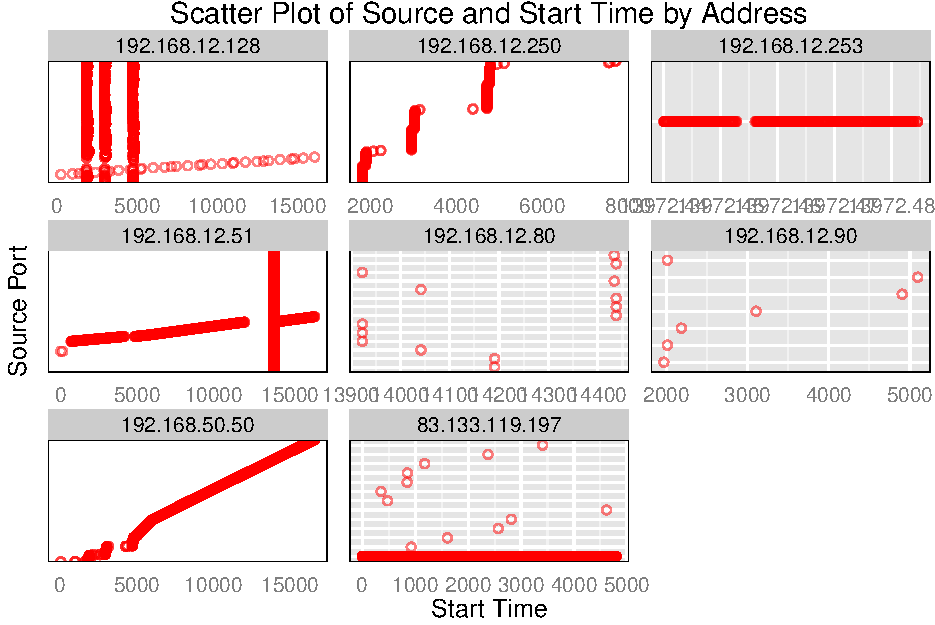
\includegraphics{edaReport_files/figure-latex/unnamed-chunk-22-1} \end{center}

\begin{center}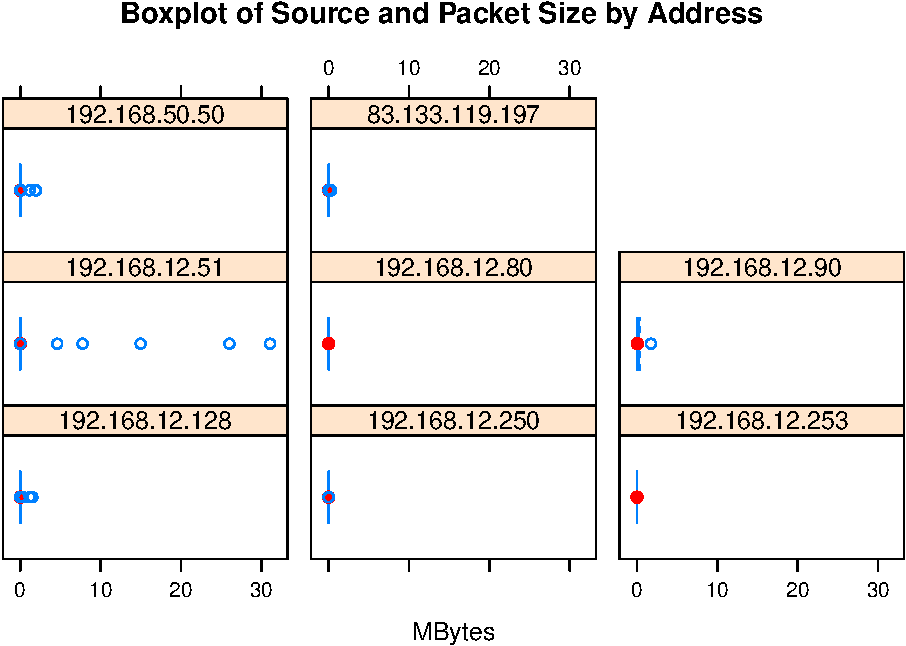
\includegraphics{edaReport_files/figure-latex/unnamed-chunk-23-1} \end{center}

\pagebreak

\begin{center}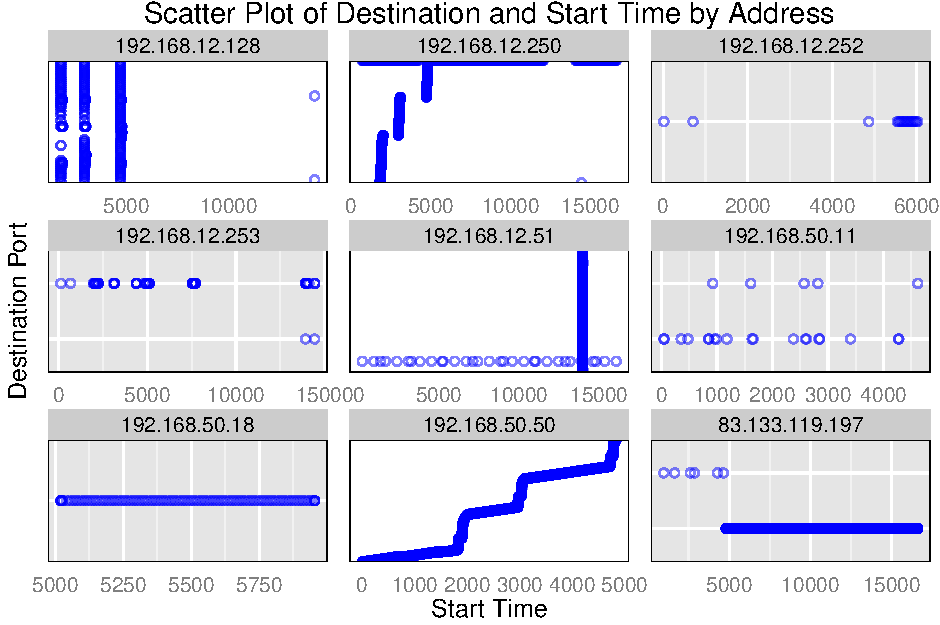
\includegraphics{edaReport_files/figure-latex/unnamed-chunk-24-1} \end{center}

\begin{center}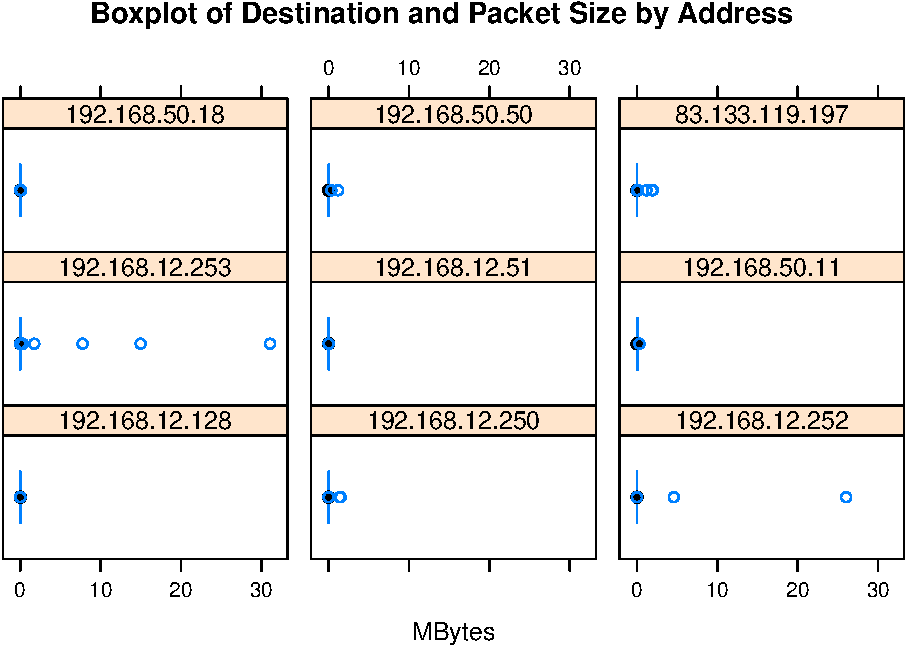
\includegraphics{edaReport_files/figure-latex/unnamed-chunk-25-1} \end{center}

\pagebreak

\begin{center}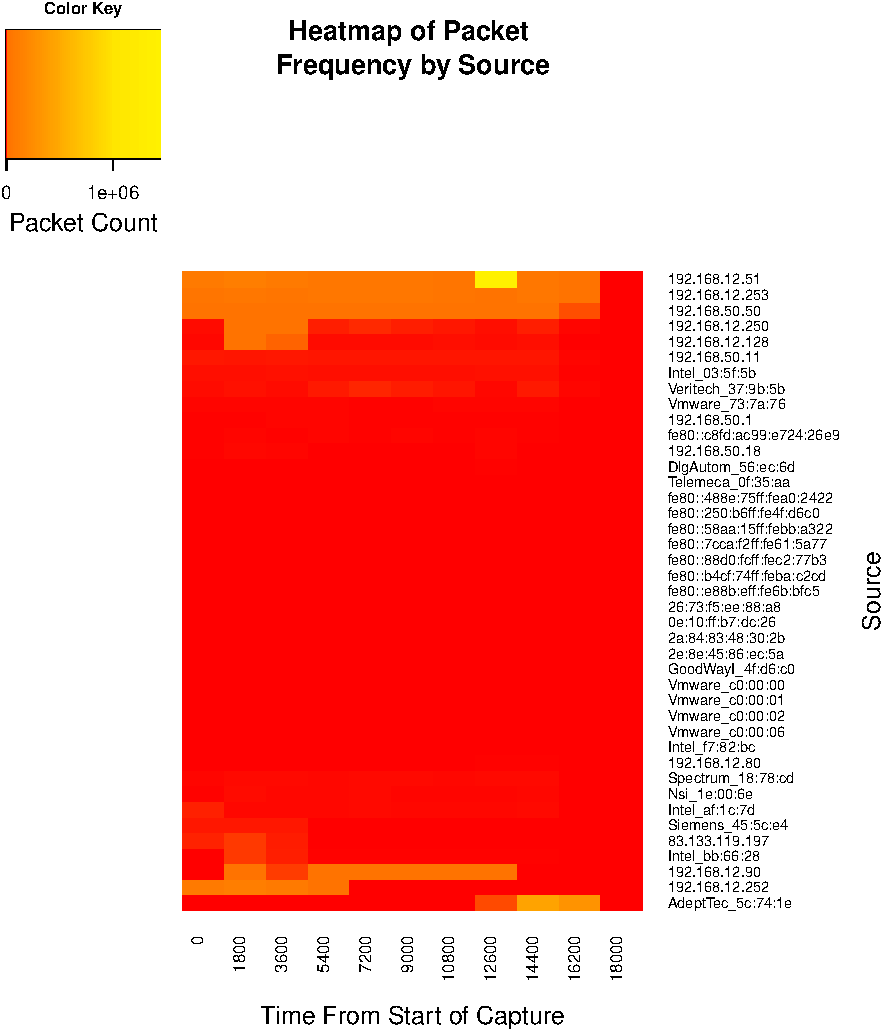
\includegraphics{edaReport_files/figure-latex/unnamed-chunk-26-1} \end{center}

\begin{center}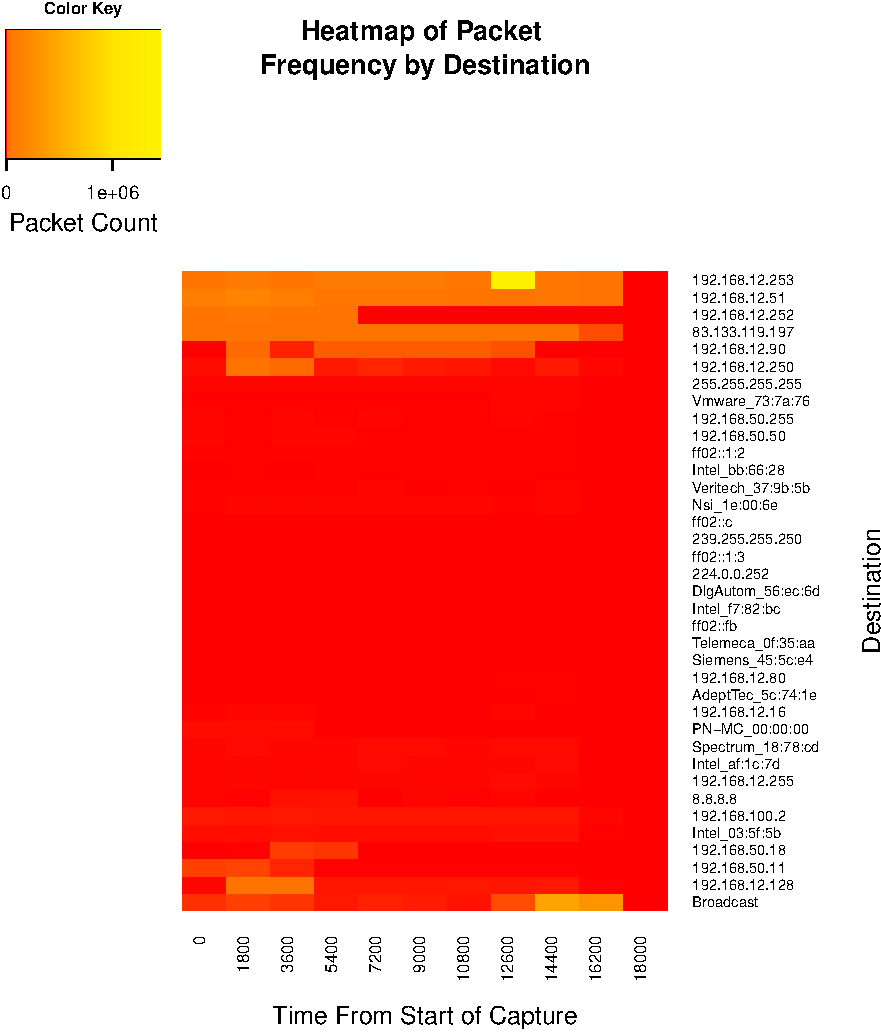
\includegraphics{edaReport_files/figure-latex/unnamed-chunk-27-1} \end{center}

\begin{center}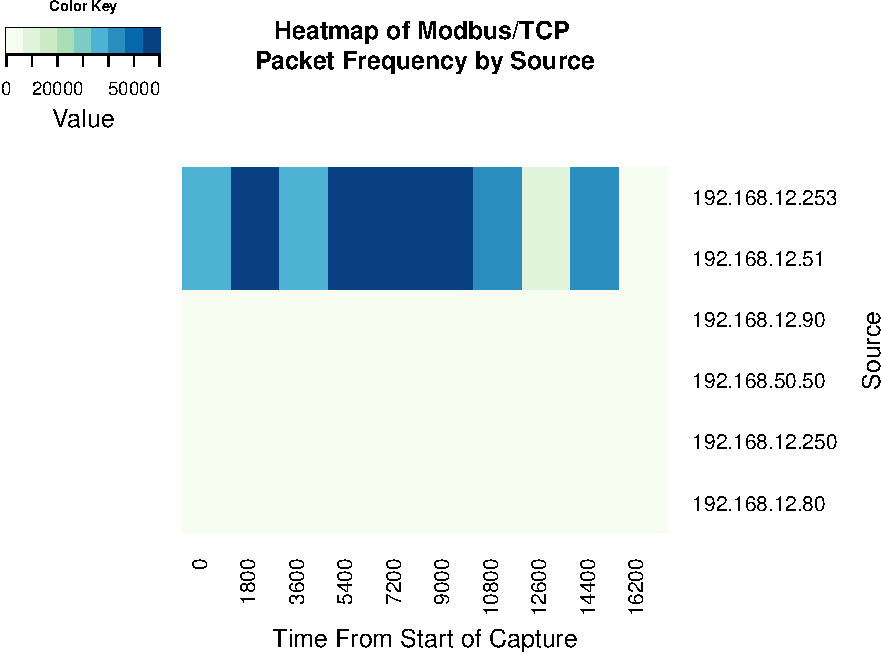
\includegraphics{edaReport_files/figure-latex/unnamed-chunk-28-1} \end{center}

\begin{center}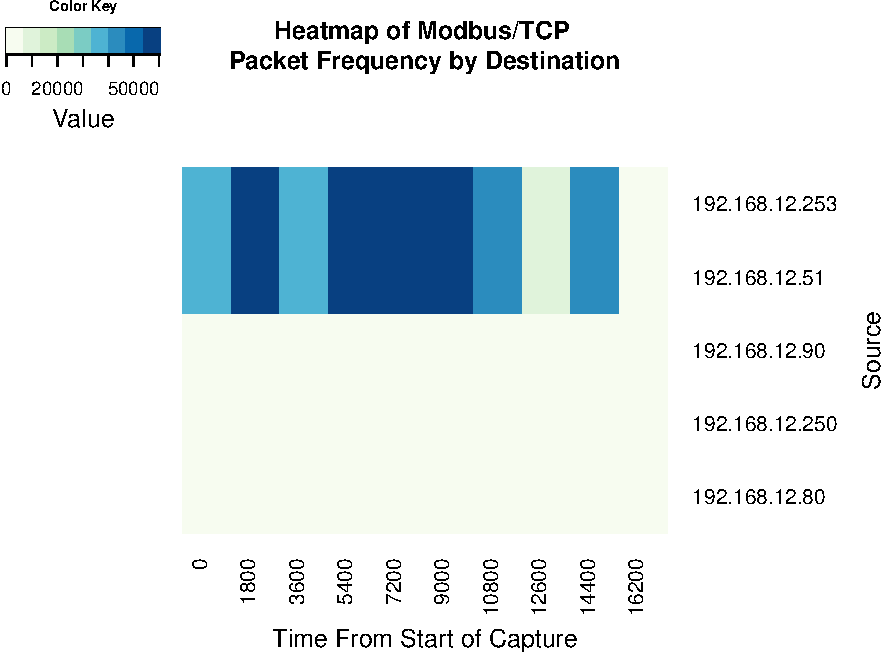
\includegraphics{edaReport_files/figure-latex/unnamed-chunk-29-1} \end{center}

\subsubsection[MODBUS/TCP Data]{MODBUS/TCP Data\footnote{\url{https://www.wireshark.org/docs/dfref/m/mbtcp.html}}}\label{modbustcp-data5}

MODBUS/TCP responses are identified by packets having source port number
502

\begin{Shaded}
\begin{Highlighting}[]
\KeywordTok{summary}\NormalTok{(responses)}
\end{Highlighting}
\end{Shaded}

\begin{verbatim}
##   frame.number     frame.time_relative frame.time_delta_displayed
##  Min.   :      1   Min.   :    0       Min.   :  0.00000         
##  1st Qu.: 215377   1st Qu.: 3705       1st Qu.:  0.00959         
##  Median : 431102   Median : 7517       Median :  0.00972         
##  Mean   : 633297   Mean   : 7622       Mean   :  0.01251         
##  3rd Qu.: 647212   3rd Qu.:10629       3rd Qu.:  0.00980         
##  Max.   :2297651   Max.   :16482       Max.   :150.30267         
##                                                                  
##    frame.len      ip.proto   ip.version            ip.src      
##  Min.   : 54.00    :     0    :     0   192.168.12.253:412780  
##  1st Qu.: 65.00   1:     0   1:     0   192.168.12.250:  1318  
##  Median : 65.00   4:     0   4:414121   192.168.12.51 :    22  
##  Mean   : 65.33   6:414121   6:     0   192.168.12.128:     1  
##  3rd Qu.: 65.00                                       :     0  
##  Max.   :315.00                         1             :     0  
##                                         (Other)       :     0  
##             ip.dst       mbtcp.modbus.unit_id  tcp.srcport    
##  192.168.12.51 :402484   Min.   :  0          502    :414121  
##  192.168.12.90 : 11188   1st Qu.:  1                 :     0  
##  192.168.12.250:   391   Median :  1          0      :     0  
##  192.168.12.80 :    37   Mean   :  1          1      :     0  
##  192.168.12.253:    21   3rd Qu.:  1          10     :     0  
##                :     0   Max.   :255          100    :     0  
##  (Other)       :     0   NA's   :1517         (Other):     0  
##   tcp.dstport     mbtcp.prot_id mbtcp.trans_id      mbtcp.len     
##  2735   :231563       :  1517   Min.   :    0.0   Min.   :  4.00  
##  2499   :111589   0   :412604   1st Qu.:   65.0   1st Qu.:  5.00  
##  3441   : 58007   1   :     0   Median :  131.0   Median :  5.00  
##  1037   :  8877   1037:     0   Mean   :  989.8   Mean   :  5.37  
##  1032   :  1646   2499:     0   3rd Qu.:  197.0   3rd Qu.:  5.00  
##  1034   :   343   4   :     0   Max.   :65313.0   Max.   :255.00  
##  (Other):  2096   502 :     0   NA's   :1517      NA's   :1517    
##  mbtcp.modbus.func_code mbtcp.modbus.reference_num mbtcp.modbus.word_cnt
##  4      :401141              :414121               Min.   : NA          
##  1      : 11140         0    :     0               1st Qu.: NA          
##         :  1517         1    :     0               Median : NA          
##  90     :   318         2    :     0               Mean   :NaN          
##  43     :     5         228  :     0               3rd Qu.: NA          
##  0      :     0         3    :     0               Max.   : NA          
##  (Other):     0         43042:     0               NA's   :414121       
##  mbtcp.modbus.data
##  00:75  :165176   
##  00:50  :155265   
##  00:54  : 33506   
##         : 12922   
##  1a:10  :  5457   
##  0a:68  :  4931   
##  (Other): 36864
\end{verbatim}

\pagebreak

MODBUS/TCP requests are identified by packets having destination port
number 502

\begin{Shaded}
\begin{Highlighting}[]
\KeywordTok{summary}\NormalTok{(requests)}
\end{Highlighting}
\end{Shaded}

\begin{verbatim}
##   frame.number     frame.time_relative frame.time_delta_displayed
##  Min.   :      2   Min.   :    0.003   Min.   :  0.0000          
##  1st Qu.: 826712   1st Qu.:13840.029   1st Qu.:  0.0001          
##  Median :1297601   Median :13886.181   Median :  0.0001          
##  Mean   :1262179   Mean   :12404.716   Mean   :  0.0060          
##  3rd Qu.:1768488   3rd Qu.:13930.370   3rd Qu.:  0.0002          
##  Max.   :2297652   Max.   :16482.127   Max.   :446.2775          
##                                                                  
##    frame.len      ip.proto    ip.version             ip.src       
##  Min.   : 54.00    :      0    :      0   192.168.12.51 :1860425  
##  1st Qu.: 54.00   1:      0   1:      0   192.168.12.90 :  22321  
##  Median : 54.00   4:      0   4:1883543   192.168.12.250:    390  
##  Mean   : 56.64   6:1883543   6:      0   192.168.50.50 :    372  
##  3rd Qu.: 54.00                           192.168.12.80 :     35  
##  Max.   :315.00                                         :      0  
##                                           (Other)       :      0  
##             ip.dst        mbtcp.modbus.unit_id  tcp.srcport     
##  192.168.12.253:1882223   Min.   :  0          2735   : 245207  
##  192.168.12.250:   1318   1st Qu.:  1          2499   : 118180  
##  192.168.12.128:      1   Median :  1          3441   :  60873  
##  192.168.12.51 :      1   Mean   :  1          1037   :  17771  
##                :      0   3rd Qu.:  1          1032   :   3306  
##  0             :      0   Max.   :255          1034   :    701  
##  (Other)       :      0   NA's   :1470635      (Other):1437505  
##   tcp.dstport      mbtcp.prot_id  mbtcp.trans_id      mbtcp.len      
##  502    :1883543       :1470635   Min.   :    0     Min.   :  4      
##         :      0   0   : 412908   1st Qu.:   65     1st Qu.:  6      
##  1      :      0   1   :      0   Median :  131     Median :  6      
##  1032   :      0   1037:      0   Mean   :  989     Mean   :  6      
##  1033   :      0   2499:      0   3rd Qu.:  197     3rd Qu.:  6      
##  1034   :      0   4   :      0   Max.   :65313     Max.   :255      
##  (Other):      0   502 :      0   NA's   :1470635   NA's   :1470635  
##  mbtcp.modbus.func_code mbtcp.modbus.reference_num mbtcp.modbus.word_cnt
##         :1470635             :1471258              Min.   :1            
##  4      : 401145        0    : 176317              1st Qu.:1            
##  1      :  11140        1    : 188770              Median :1            
##  90     :    618        2    :  23602              Mean   :1            
##  43     :      5        228  :      0              3rd Qu.:1            
##  0      :      0        3    :  23596              Max.   :1            
##  (Other):      0        43042:      0              NA's   :1482398      
##  mbtcp.modbus.data 
##          :1883220  
##  01:04   :     84  
##  00:04   :     52  
##  00:01:00:     34  
##  00:02   :     34  
##  01:12   :     32  
##  (Other) :     87
\end{verbatim}

MODBUS function codes requested:

\begin{Shaded}
\begin{Highlighting}[]
\KeywordTok{table}\NormalTok{(moddataDT[,mbtcp.modbus.func_code])}
\end{Highlighting}
\end{Shaded}

\begin{verbatim}
## 
##               0       1       2     228       4   42786      43      90 
## 1472139       7   22280       2       1  802286       2      10     936
\end{verbatim}

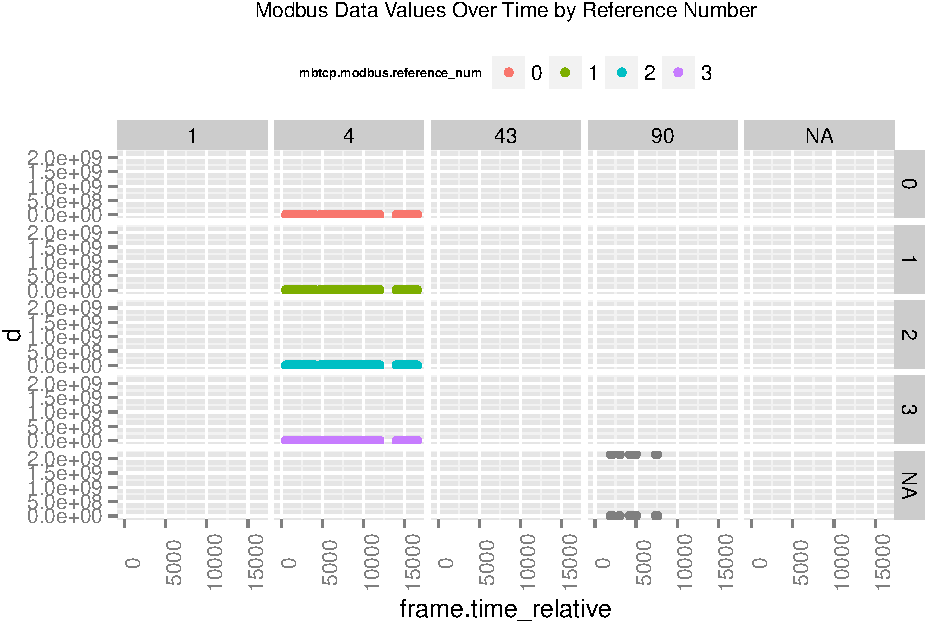
\includegraphics{edaReport_files/figure-latex/unnamed-chunk-35-1.pdf}

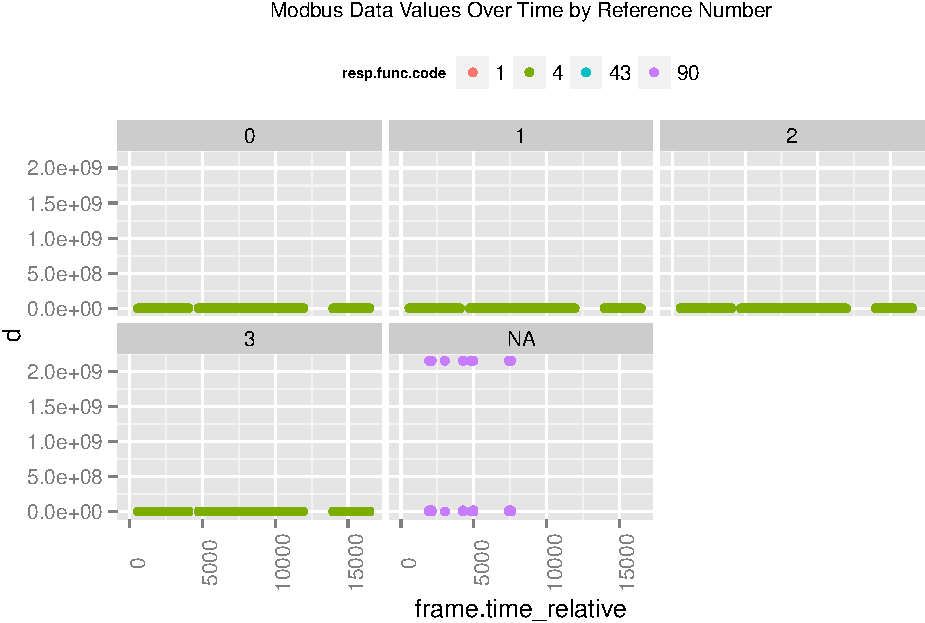
\includegraphics{edaReport_files/figure-latex/unnamed-chunk-36-1.pdf}

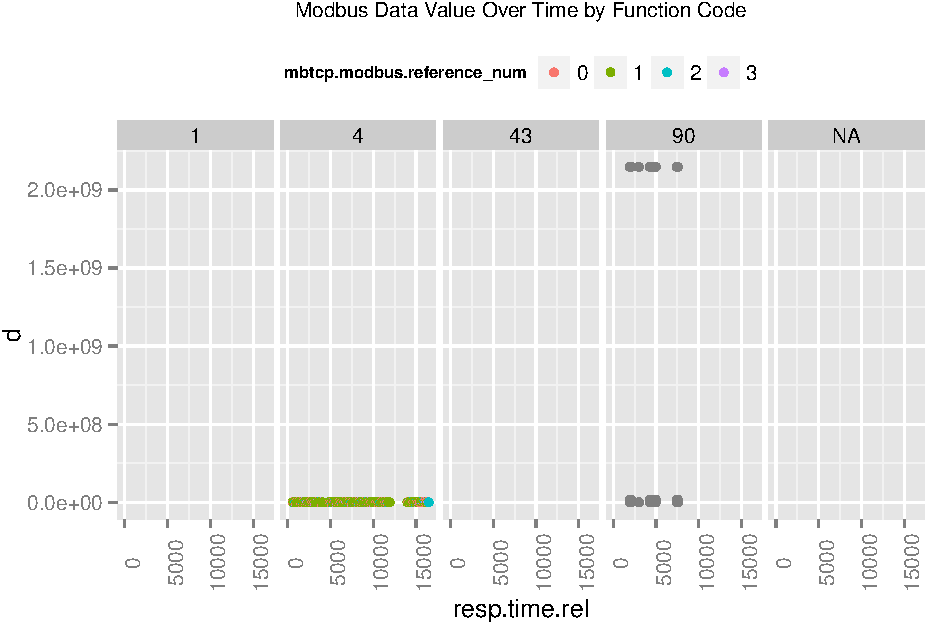
\includegraphics{edaReport_files/figure-latex/unnamed-chunk-37-1.pdf}

\pagebreak

\begin{Shaded}
\begin{Highlighting}[]
\KeywordTok{summary}\NormalTok{(mergedDT)}
\end{Highlighting}
\end{Shaded}

\begin{verbatim}
##   frame.number     frame.time_relative frame.time_delta_displayed
##  Min.   :      0   Min.   :    0       Min.   :0.000             
##  1st Qu.: 214962   1st Qu.: 3699       1st Qu.:0.000             
##  Median : 431188   Median : 7518       Median :0.000             
##  Mean   : 637759   Mean   : 7631       Mean   :0.015             
##  3rd Qu.: 648965   3rd Qu.:10654       3rd Qu.:0.000             
##  Max.   :2297650   Max.   :16482       Max.   :1.233             
##  NA's   :9081      NA's   :9081        NA's   :9081              
##    frame.len                 ip.src                  ip.dst      
##  Min.   :  0.00                 :   158                 :   158  
##  1st Qu.: 66.00   192.168.12.250:    12   192.168.12.253:403523  
##  Median : 66.00   192.168.12.51 :395531   NA's          :  9081  
##  Mean   : 65.98   192.168.12.80 :     4                          
##  3rd Qu.: 66.00   192.168.12.90 :  7781                          
##  Max.   :315.00   192.168.50.50 :   195                          
##  NA's   :9081     NA's          :  9081                          
##   tcp.srcport     tcp.dstport   mbtcp.prot_id mbtcp.trans_id   
##  2735   :227139   502 :403523   0   :403523   Min.   :    0.0  
##  2499   :110386   NA's:  9239   NA's:  9239   1st Qu.:   65.0  
##  3441   : 58006                               Median :  131.0  
##  1037   :  6447                               Mean   :  989.4  
##  1032   :  1102                               3rd Qu.:  197.0  
##  (Other):   443                               Max.   :65313.0  
##  NA's   :  9239                                                
##    mbtcp.len       mbtcp.modbus.func_code mbtcp.modbus.word_cnt
##  Min.   :  0.000   1   :  7770            Min.   :0            
##  1st Qu.:  6.000   4   :395531            1st Qu.:1            
##  Median :  6.000   43  :     4            Median :1            
##  Mean   :  6.005   90  :   218            Mean   :1            
##  3rd Qu.:  6.000   NA's:  9239            3rd Qu.:1            
##  Max.   :255.000                          Max.   :1            
##  NA's   :9081                             NA's   :17073        
##  mbtcp.modbus.reference_num resp.fr.number    resp.time.rel  
##  0   :170489                Min.   :      0   Min.   :    0  
##  1   :186219                1st Qu.: 215350   1st Qu.: 3704  
##  2   : 23375                Median : 431230   Median : 7518  
##  3   : 23218                Mean   : 634753   Mean   : 7625  
##  NA's:  9461                3rd Qu.: 647762   3rd Qu.:10636  
##                             Max.   :2297651   Max.   :16482  
##                             NA's   :3450      NA's   :3450   
##  resp.time.delta    resp.len                resp.src     
##  Min.   :0.000   Min.   :  0.00                 :   158  
##  1st Qu.:0.010   1st Qu.: 65.00   192.168.12.253:409154  
##  Median :0.010   Median : 65.00   NA's          :  3450  
##  Mean   :0.011   Mean   : 65.32                          
##  3rd Qu.:0.010   3rd Qu.: 65.00                          
##  Max.   :0.119   Max.   :315.00                          
##  NA's   :3450    NA's   :3450                            
##           resp.dest      resp.srcport   resp.dstport    resp.prot_id 
##                :   158   502 :409154   2735   :229397   0   :409154  
##  192.168.12.250:   284   NA's:  3608   2499   :111014   NA's:  3608  
##  192.168.12.51 :398417                 3441   : 58006                
##  192.168.12.80 :     4                 1037   :  8553                
##  192.168.12.90 : 10449                 1032   :  1550                
##  NA's          :  3450                 (Other):   634                
##                                        NA's   :  3608                
##  resp.trans_id     resp.mbcp.len     resp.func.code   resp.data     
##  Min.   :    0.0   Min.   :  0.000   1   : 10432    00:75  :163854  
##  1st Qu.:   65.0   1st Qu.:  5.000   4   :398417    00:50  :154306  
##  Median :  131.0   Median :  5.000   43  :     5    00:54  : 33278  
##  Mean   :  989.4   Mean   :  5.347   90  :   300           : 10841  
##  3rd Qu.:  197.0   3rd Qu.:  5.000   NA's:  3608    1a:10  :  5431  
##  Max.   :65313.0   Max.   :255.000                  (Other): 41602  
##                    NA's   :3450                     NA's   :  3450  
##        d            
##  Min.   :8.000e+01  
##  1st Qu.:8.000e+01  
##  Median :1.170e+02  
##  Mean   :8.171e+04  
##  3rd Qu.:1.170e+02  
##  Max.   :2.147e+09  
##  NA's   :14291
\end{verbatim}

\pagebreak

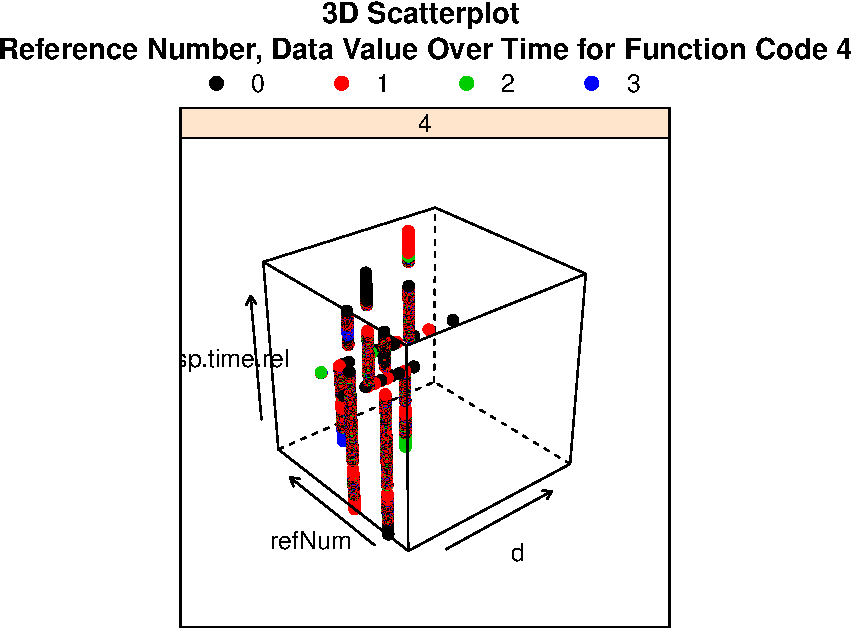
\includegraphics{edaReport_files/figure-latex/unnamed-chunk-40-1.pdf}

\begin{Shaded}
\begin{Highlighting}[]
\NormalTok{mergedDT[,.(}\DataTypeTok{count=}\NormalTok{.N, }\DataTypeTok{d.min=}\KeywordTok{min}\NormalTok{(d), }\DataTypeTok{d.mean=}\KeywordTok{mean}\NormalTok{(d, }\DataTypeTok{na.rm=}\NormalTok{T), }\DataTypeTok{d.max=}\KeywordTok{max}\NormalTok{(d),}
            \DataTypeTok{d.sd=}\KeywordTok{sd}\NormalTok{(d, }\DataTypeTok{na.rm=}\NormalTok{T), }\DataTypeTok{min.resp.time.rel=}\KeywordTok{min}\NormalTok{(resp.time.rel),}
            \DataTypeTok{min.resp.time.rel=} \KeywordTok{max}\NormalTok{(resp.time.rel)), }
         \NormalTok{by =.(resp.func.code, mbtcp.modbus.reference_num)][}
           \KeywordTok{order}\NormalTok{(resp.func.code, mbtcp.modbus.reference_num)]}
\end{Highlighting}
\end{Shaded}

\begin{verbatim}
##     resp.func.code mbtcp.modbus.reference_num  count d.min       d.mean
##  1:              1                          0   7769    NA          NaN
##  2:              1                         NA   2663    NA          NaN
##  3:              4                          0 162720   117 1.170000e+02
##  4:              4                          1 186219    80 8.070932e+01
##  5:              4                          2  23375  1325 3.638839e+03
##  6:              4                          3  23218  1726 4.726736e+03
##  7:              4                         NA   2885    80 6.398964e+02
##  8:             43                         NA      5    NA          NaN
##  9:             90                         NA    300    NA 5.986910e+08
## 10:             NA                         NA   3608    NA          NaN
##     d.max         d.sd min.resp.time.rel min.resp.time.rel
##  1:    NA           NA         1834.1548         13840.532
##  2:    NA           NA         1877.1583         13839.574
##  3:   117 0.000000e+00          572.0978         16479.497
##  4:    84 1.527791e+00          572.1377         16480.157
##  5:  5136 9.848511e+02          572.0877         16482.127
##  6:  9350 1.969740e+03          572.1577         16479.167
##  7:  6680 1.511860e+03         1877.0379         11873.525
##  8:    NA           NA         1877.0490         14303.061
##  9:    NA 9.695551e+08         1877.0571          7586.738
## 10:    NA           NA                NA                NA
\end{verbatim}

\pagebreak

\section{References}\label{references}

{[}1{]} L. Maliphol, \href{mailto:SCAD@COPS}{\nolinkurl{SCAD@COPS}}: A
Hybrid Network Intrusion Detection System

{[}2{]} J.W. Tukey, (1977). Exploratory Data Analysis. Addison-Wesley.
ISBN 0-201-07616-0

{[}3{]} P. Lafaye de Micheaux et al., (2013). The R Software:
Fundamentals of Programming and Statistical Analysis, Statistics and
Computing. Springer New York. ISBN 978-1-4614-9019-7

\pagebreak

\section{Appendix A}\label{appendix-a}

Using the export facility in Wireshark, the following are a description
of the exported files:

Entire pcap file exported in CSV format:

\begin{longtable}[c]{@{}l@{}}
\toprule
SCADA\_20150429\_042915.csv\tabularnewline
\midrule
\endhead
Time\tabularnewline
Source\tabularnewline
Destination\tabularnewline
Protocol\tabularnewline
Length\tabularnewline
Info\tabularnewline
\bottomrule
\end{longtable}

List of endpoints, the traffic to and from an IP address:

\begin{longtable}[c]{@{}l@{}}
\toprule
SCADA\_Security\_042915\_TCP\_Endpoints.csv\tabularnewline
\midrule
\endhead
Address\tabularnewline
Port\tabularnewline
Packets\tabularnewline
Bytes\tabularnewline
Tx.Packets\tabularnewline
Tx.Bytes\tabularnewline
Rx.Packets\tabularnewline
Rx.Bytes\tabularnewline
Latitude\tabularnewline
Longitude\tabularnewline
\bottomrule
\end{longtable}

List of conversations, the traffic between two endpoints :

\begin{longtable}[c]{@{}l@{}}
\toprule
SCADA\_Security\_042915\_TCP\_Conversations.csv\tabularnewline
\midrule
\endhead
Address.A\tabularnewline
Port.A\tabularnewline
Address.B\tabularnewline
Port.B\tabularnewline
Packets\tabularnewline
Bytes\tabularnewline
Packets.A.B\tabularnewline
Bytes.A.B\tabularnewline
Packets.A.B.1\tabularnewline
Bytes.A.B.1\tabularnewline
Rel.Start\tabularnewline
Duration\tabularnewline
bps.A.B\tabularnewline
bps.A.B.1\tabularnewline
\bottomrule
\end{longtable}

\pagebreak

\section{Appendix B}\label{appendix-b}

\subsection{Commands and Scripts}\label{commands-and-scripts}

\subsubsection{TShark}\label{tshark}

Command used to extract various fields from the pcap file used for
analysis.

tshark -r modbus.pcap -T fields -E separator=, -t r -E header=y -e
frame.number -e frame.time\_relative -e frame.time\_delta\_displayed -e
frame.len -e ip.proto -e ip.version -e ip.src -e ip.dst -e
mbtcp.modbus.unit\_id -e tcp.srcport -e tcp.dstport -e mbtcp.prot\_id -e
mbtcp.trans\_id -e mbtcp.len -e mbtcp.modbus.func\_code -e
mbtcp.modbus.reference\_num

-e mbtcp.modbus.word\_cnt -e mbtcp.modbus.data \textgreater{}
modbus.data

\subsubsection{sed}\label{sed}

Command used to remove empty lines from the pcap data.

sed '/\^{},.*\$/d' modbus.data \textgreater{} modbus.data

\subsubsection{R}\label{r}

install.R - Setup script to install required packages. scada.R - Script
in the language R containing for conducting statistical analysis and
creating graphic visualisations. modVals.R - Script for processing and
analysing modbus data packets.

\end{document}
